\section{Results and discussion}

\begin{figure*}
	\centering
	\begin{subfigure}{1\linewidth}
		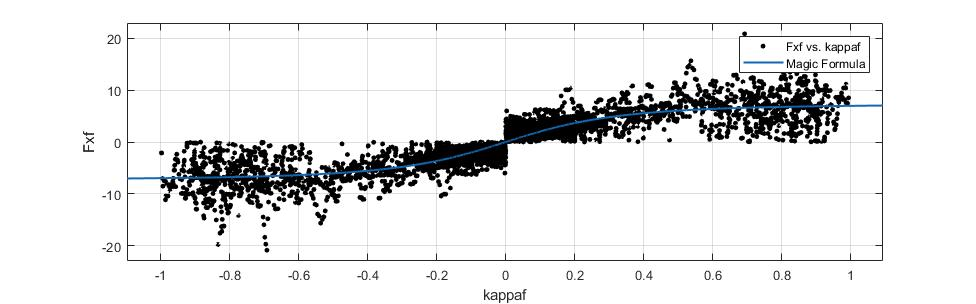
\includegraphics[scale=0.52]{figure/MagicFormulaFrontBags}
		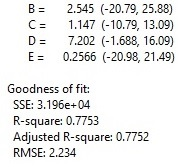
\includegraphics[scale=1.1]{figure/MagicFormulaFrontBagsFitnumbers}
		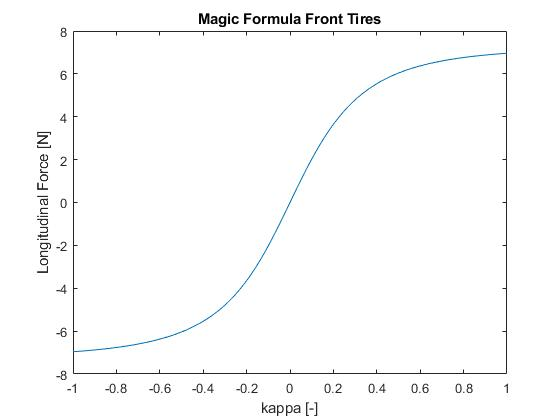
\includegraphics[scale=0.4]{figure/MagicFormulaFrontBagsPic}
        \caption{The front wheels}
    \label{fig:mffront}
\end{subfigure}
	\begin{subfigure}{1\linewidth}
		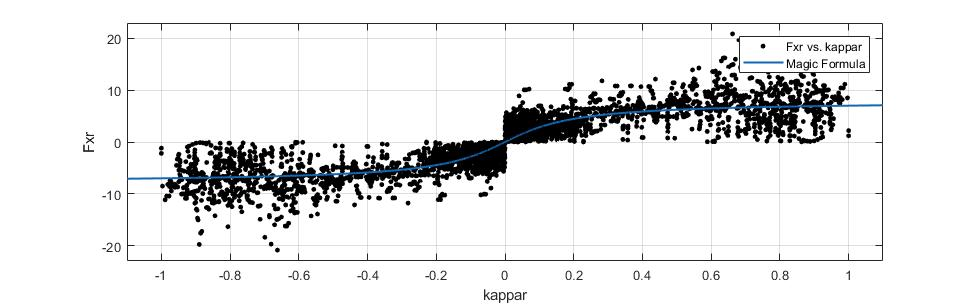
\includegraphics[scale=0.52]{figure/MagicFormulaRearBags}
		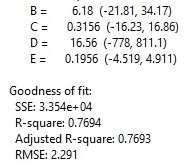
\includegraphics[scale=1.1]{figure/MagicFormulaRearBagsFitnumbers}
		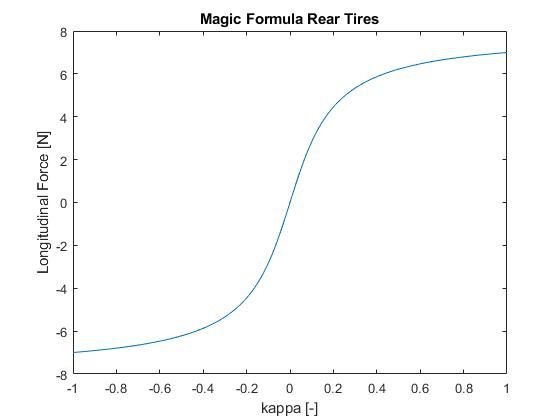
\includegraphics[scale=0.4]{figure/MagicFormulaRearBagsPic}
		
        \caption{The rear wheels}
        \label{fig:mfrear}
    \end{subfigure}
    \caption{Fitted Magic Formula's from combined data}
    \label{fig:mf}
\end{figure*}
\begin{figure}
	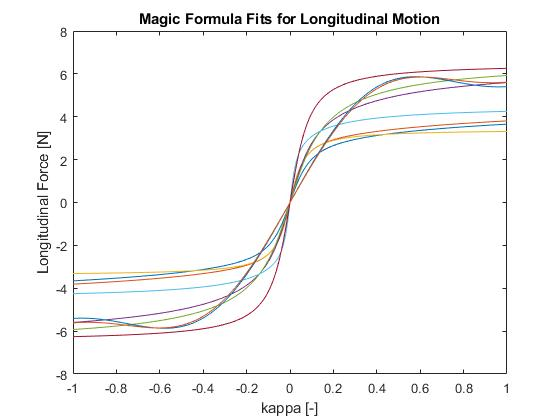
\includegraphics[scale=0.4]{figure/SeperateBags.jpg}
    \caption{Fitted Magic formulas for separate tests}
    \label{fig:MagicFormulaSplit}
\end{figure}
As noticeable from the plots, the Magic Formula does not take its regular form. Even though there are comparisons with the Magic Formula, it still is not what was expected. First of all, the Magic Formula has a peak and descends afterwards. This is not the case with Figures \ref{fig:mf}\subref{fig:mffront} and \ref{fig:mf}\subref{fig:mfrear}. Secondly, most magic formulas ascend much faster than our Magic Formula. 
	There are a few possibilities why our Magic Formula differs from others. First of all, the peak in the Magic Formula (Figure \ref{fig:MagicFit}) is related to tire stiffness. As the tire stiffness increases the peak decreases \cite{Jonson}. As our plastic rims with grip tape approach infinite stiffness when compared to air inflated tires, this peak is very small or does not exist. 
    
A second possibility can be the data given by the Tachometers. The sampling time of ROS is much faster than the sampling time of the Hall sensors. This results in many data points where no revolution is detected. Therefore, this data contains a lot of zeros.  Because of this, interpolation between non-zero values is needed. This can result in inaccurate data.
    
Another possible reason  can be varying tire conditions. Through the process of experimenting, wear definitely occurred. Also heat can have effect on the behavior of these tires. Therefore it is possible that the changing tire conditions led to a less accurate Magic Formula. 
The last possibility can be due to noise generated by the IMU. Looking at figures \ref{fig:mf}\subref{fig:mffront} and \ref{fig:mf}\subref{fig:mfrear} we see a lot of noise in our plots, even with the help of the filters that were used. There are three possible contributions to this noise. First is the RC car we used. As the first aim was to improve the data acquisition software, not much was changed about the car itself. It was not after much testing was done before it became clear that the wheels were not balanced very well. This resulted in many vibrations. Especially the IMU (Inertial Measurement Unit) generated much noise because of this. The second possible explanation is that the IMU has not been properly calibrated. This has proven to be very difficult due to the complexity of the code of the IMU. Lastly, the IMU could not be installed perfectly normal to the floor.

However, the goodness of the fits for the combined experiments of the front and rear tires are decent, around 0.77. Goodness of fit becomes even higher when fitting the Magic Formula for some separate tests, varying between 0.80 and 0.93. The most plausible explanation for the difference between the plots in Figure \ref{fig:MagicFormulaSplit} is that the condition of the tires varies between measurements. Also, the shapes of our plots show comparison with the Magic Formula. This suggests that determining tire characteristics with the help of this experimental setup is heading towards the good direction. With some adjustments, this method can be very useful for determining tire characteristics.

Finally, the magic formula for the slip angles are missing. This is because the dynamixel was not functioning properly. Therefore, the steering angles could not be determined accurately enough to generate proper data. However, if the dynamixel is installed correctly and proper data is generated, it should be easy to determine the magic formula for the slip angles with the method described in this paper.

